\documentclass{article}
\usepackage[utf8]{inputenc}

\title{Modern Computer Architecture\\Lab Report}
\author{%
    Mick van Gelderen\\4091566
    \and
    Arian Stolwijk\\4001079
}

\date{November 2013}

\usepackage{natbib}
\usepackage{graphicx}
\usepackage{listings}

\begin{document}

\newcommand{\rvex}{\ensuremath{\rho}-VEX}
\newcommand{\satd}{\texttt{x264\_pixel\_satd\_8x4}}
\newcommand{\getref}{\texttt{get\_ref}}

\maketitle

\section{The kernel function}

The concept of this lab is to take a piece of code that is executed frequently
and run it on a reconfigurable co-processor. The extracted piece of code is
called the kernel and the device is in our case the \rvex{}: A reconfigurable
and extensible VLIW processor.

The kernel needs to be compiled for the \rvex{} so that we can inject the
result, the bytecode, in to the co-processor. The rest of the code runs as
usual on a regular processor.

\section{Communication}

We have access to several (but not enough during the lab) FPGAs which are
configured as Microblaze processors and run Linux.

The \rvex{} is a configured as a co-processor that can be controlled using a
number of memory mapped files.  The is a file for writing the instruction
memory, one for reading and writing the data memory, one for reading the status
and one for writing control commands.

We abstracted this away to a small interface with the following functionality:

\begin{description}
    \item[rvexInit] \hfill \\
        Attempts to open the files.
    \item[rvexDispose] \hfill \\
        Closes all files opened by rvexInit.
    \item[rvexBytecode] \hfill \\
        Allows you to write bytecode to the instruction memory.
    \item[rvexWrite] \hfill \\
        Allows you to write to the data memory.
    \item[rvexRead] \hfill \\
        Allows you to read from the data memory.
    \item[rvexSeek] \hfill \\
        Allows you to jump to a given position in the data memory.
    \item[rvexGo] \hfill \\
        Writes the clear and start commands to the control memory and blocks until the status reports that the operation was successful.
\end{description}

\section{Profiling results}

We compiled the unmodified x264 application with profiling support on a VM that
allows us to compile microblaze and \rvex{} applications. Unfortunately we
cannot use gprof on the Microblaze machine itself so we ran gprof on the VM
itself.

	Using the input video $\sim$/Videos/inputs/eledream\_640x360\_8.y4m we obtained
the following profiling results.

\begin{small}\begin{lstlisting}
gprof x264 | head -n 10
Flat profile:

Each sample counts as 0.01 seconds.
  %   cumulative   self              self     total
 time   seconds   seconds    calls  ms/call  ms/call  name
 13.70      0.10     0.10  1599044     0.00     0.00  x264_pixel_satd_8x4
 13.70      0.20     0.10   570708     0.00     0.00  get_ref
  6.85      0.25     0.05    38770     0.00     0.00  x264_pixel_sad_x4_16x16
  5.48      0.29     0.04   460484     0.00     0.00  quant_4x4
  4.11      0.32     0.03   123076     0.00     0.00  sa8d_8x8
\end{lstlisting}\end{small}

We see that the function \satd{} is called 1.6 million times during the video
conversion. These calls together take up about $14\%$ of the total time. An
equal amount of time is spend in \satd{}.

The video eledream\_640x360\_128.y4m makes the application spend about $18\%$
of the runtime in the pixel processing function and $16\%$ in \getref{}.

The bigger our input video the more time we will spend processing and the more
effect an optimization will have if it targets part of the processing code.

Judging from the profiling information there are two potential places where
optimization will be effective: \satd{} and \getref{}.

When we looked at the source code of x264 we thought that the nature of \satd{}
was more suitable for optimization because it had some loops in it. The
\getref{} function was a lot more irregular and also harder to understand. On
the flip side, the overhead caused by communication between the microblaze
processor and the \rvex{} would be smaller for \getref{} because it is called
three times less than \satd{}.

In the end we chose to try and put the computation of \satd{} on the
co-processor and let \getref{} for what it was. The function \satd{} was easier
to understand and making it work was more important to us than choosing the
best optimization area right away.

\section{Endianess}

Since we had to compile for the Microblaze using the flag -DWORD-BIGENDIAN we
figured that the Microblaze would be a big endian machine. You can always test
it by writing a multibyte value like 0xDEADBEEF to memory and read the
individual bytes. If you read 0xDE 0xAD 0xBE 0xEF you will know that you have a
big endian machine. If you get that sequence but in reverse you know its a
little endian machine.

\section{Results of using the \rvex{}}

We modified the x264 application to log its processing time computed with
clock\_gettime. This required linking the rt library.

Then we tried to find an fpga that was not being used by anyone else and we ran
the application.

\begin{tabular}{ l c r }
  1 & 2 & 3 \\
  4 & 5 & 6 \\
  7 & 8 & 9 \\
\end{tabular}

\begin{itemize}
  \item How much speedup did you obtain?
  \item Is this what you have expected?
  \item Give a theoretical calculation for the speedup you should have ex-
        pected and compare it to the practical result.
\end{itemize}

\section{Additional assignment}

\begin{itemize}
  \item What were the results of the additional assignment? How did it affect
        the speed of the application?
\end{itemize}

\begin{figure}[h!]
  \centering
  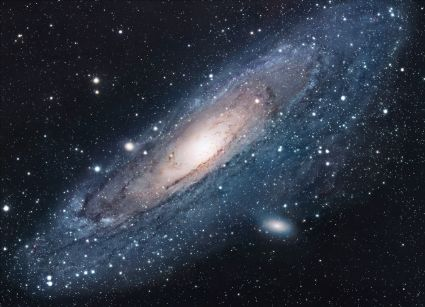
\includegraphics[scale=1.7]{universe.jpg}
  \caption{The Universe}
  \label{threadsVsSync}
\end{figure}

\section{Conclusion}

``I always thought something was fundamentally wrong with the universe'' \citep{adams1995hitchhiker}

\bibliographystyle{plain}
\bibliography{main}

\end{document}

